\documentclass[arhiv]{izpit}
\usepackage{fouriernc}

\begin{document}

\izpit{Programiranje I: 1. izpit}{3. februar 2011}{
  Čas reševanja je 120 minut.
  Veliko uspeha!
}

\naloga[25 točk]

Pri programiranju obstaja več pristopov k zapisu dolgih imen
spremenljivk. Nekateri pišejo \verb|dolgoImeSpremenljivke|, drugi pa
\verb|dolgo_ime_spremenljivke|.
  
\podnaloga
%
Sestavite funkcijo \verb|pobrisiPodcrtaje|, ki sprejme ime
spremenljivke s podčrtaji in malimi začetnicami ter vrne pripadajoče
ime brez podčrtajev in z velikimi začetnicami. Primer uporabe:
%
\begin{verbatim}
>>> pobrisiPodcrtaje("dolgo_ime_spremenljivke")
"dolgoImeSpremenljivke"
\end{verbatim}

    % def pobrisiPodcrtaje(ime):
    %     besede = ime.split("_")
    %     return besede[0] + "".join(beseda.capitalize() for beseda in besede[1:])
  
\podnaloga
%
Sestavite funkcijo \verb|dodaj_podcrtaje|, ki deluje ravno obratno kot
\verb|pobrisiPodcrtaje|. Primer uporabe:
\begin{verbatim}
>>> dodaj_podcrtaje("dolgoImeSpremenljivke")
"dolgo_ime_spremenljivke"
\end{verbatim}

    % def pobrisiPodcrtaje(ime):
    %     besede = ime.split("_")
    %     return besede[0] + "".join(beseda.capitalize() for beseda in besede[1:])

    % def dodajPodcrtaje(ime):
    %     def popraviZacetnico(m):
    %         return "_" + m.group(0).lower()
    %     return re.sub("[A-Z]", popraviZacetnico, ime)

\naloga[25 točk]

\emph{Izbor reda $n$} je strogo naraščajoče zaporedje naravnih števil,
ki so vsa med $1$ in $n$. Na primer, $[1,2,3,7]$ je izbor reda $9$ in
\emph{ni} izbor reda $5$. Vsi izbori reda~$2$ so $[\,]$, $[1]$, $[2]$,
in $[1,2]$.
%
Sestavite generator \verb|izbori(n)|, ki zgenerira vse izbore reda \verb|n|.

% def izbori(n, k = 1):
%     if k > n:
%         yield []
%     else:
%         for izbor in izbori(n, k + 1):
%             yield izbor
%             yield [k] + izbor

\naloga[25 točk]

Na spletni učilnici najdete datoteko \verb|IskalnoDrevo.py|, v kateri
je dan razred iskalnih dreves.

\podnaloga
%
Razredu dodajte metodo
\verb|predhodnik(self, x)|, ki vrne največji element v drevesu
\verb|self|, ki je še strogo manjši od \verb|x|. Na primer, če so v drevesu
\verb|d| shranjena števila $1$, $3$, $5$, $10$, $12$, potem ukaz
\verb|d.predhodnik(9)| vrne $5$.

% def predhodnik(self, x):
%     if self.prazno:
%         return None
%     elif x <= self.vsebina:
%         return self.levo.predhodnik(x)
%     else: # self.vsebina < x
%         y = self.desno.predhodnik(x)
%         return (y or self.vsebina)

\podnaloga[+10 točk]
%
Sestavite še metodo \verb|interval(self, x, y)|, ki vrne seznam tistih
elementov v drevesu, ki so strogo večji od \verb|x| in strogo manjši
od \verb|y|.

% def interval(self, x, y):
%     if self.prazno:
%         return []
%     else:
%         a = self.levo.interval(x,y)
%         if x < self.vsebina < y:
%             a.append(self.vsebina)
%         a.extend(self.desno.interval(x,y))
%         return a

\naloga[25 točk]

Iz pravokotnika velikosti $v \times s$ lahko ustvarimo naključen
labirint po naslednjem postopku:
\begin{itemize}
\item Če je bodisi višina $v$ bodisi širina $s$ enaka $1$, končamo.
\item Če je višina $v$ manjša od širine $s$:
  \begin{enumerate}
  \item Izberemo naključen $x \in \{1, \dots, s - 1\}$.
  \item Izberemo naključen $y \in \{0, \dots, v - 1\}$.
  \item Pravokotnik predelimo na pol s črtama od točke $(x, 0)$ do točke
    $(x, y)$ ter od točke $(x, y + 1)$ do točke $(x, v)$.
  \item Postopek ponovimo na levi polovici.
  \item Postopek ponovimo na desni polovici.
  \end{enumerate}
  \[
  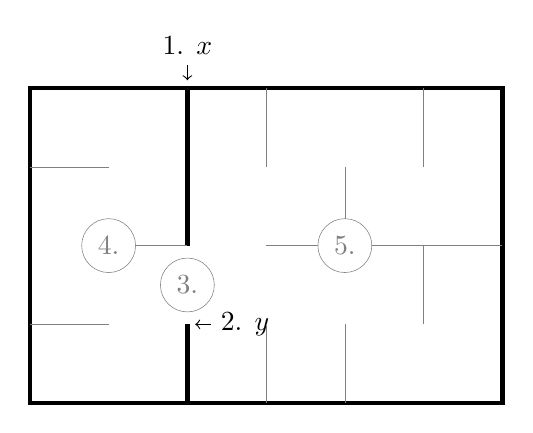
\begin{tikzpicture}
    \draw[ultra thick] (0, 0) rectangle (6, 4);
    \draw[<-] (2, 4.1) -- (2, 4.3) node[anchor=south] {1. $x$};
    \draw[<-] (2.1, 1) -- (2.3, 1) node[anchor=west] {2. $y$};
    \draw[ultra thick] (2, 0) -- (2, 1) (2, 2) -- (2, 4);
    \draw (2, 1.5) node[draw, circle, help lines, fill=white] {3.};
    
    \draw[help lines]
    (1, 2) node[draw, circle, fill=white] {4.}
    (0, 3) -- (1, 3)
    (1, 2) -- (2, 2)
    (0, 1) -- (1, 1);
    \draw[help lines]
    (4, 2) node[draw, circle, fill=white] {5.}
    (3, 2) -- (6, 2)
    (4, 2) -- (4, 3)
    (5, 2) -- (5, 1)
    (3, 0) -- (3, 1)
    (4, 0) -- (4, 1)
    (3, 3) -- (3, 4)
    (5, 3) -- (5, 4)
    ;
  \end{tikzpicture}
  \]
\item Če je višina $v$ ni manjša od širine $s$, ravnamo podobno, le da
  pravokotnik predelimo po višini.
\end{itemize}

  V \emph{Mathematici} sestavite funkcijo \texttt{labirint[v\_, s\_]}, ki po
  zgornjem postopku sestavi na\-klju\-čen labirint iz ustreznih grafičnih ukazov.

  % predeliLabirint[1, _, _, _] = {};
  % predeliLabirint[_, 1, _, _] = {};
  % predeliLabirint[v_, s_, x0_, y0_] :=
  %  If[v < s,
  %   With[
  %    {
  %     x = RandomInteger[{1, s - 1}],
  %     y = RandomInteger[{0, v - 1}]
  %    },
  %    {
  %     Line[{{x0 + x, y0}, {x0 + x, y0 + y}}],
  %     Line[{{x0 + x, y0 + y + 1}, {x0 + x, y0 + v}}],
  %     predeliLabirint[v, x, x0, y0],
  %     predeliLabirint[v, s - x, x0 + x, y0]
  %     }
  %    ],
  %    With[
  %     {
  %      y = RandomInteger[{1, v - 1}],
  %      x = RandomInteger[{0, s - 1}]
  %     },
  %     {
  %      Line[{{x0, y0 + y}, {x0 + x, y0 + y}}],
  %      Line[{{x0 + x + 1, y0 + y}, {x0 + s, y0 + y}}],
  %      predeliLabirint[y, s, x0, y0],
  %      predeliLabirint[v - y, s, x0, y0 + y]
  %      }
  %     ]
  %   ]
  % 
  % labirint[v_, s_] :=
  %  Graphics[
  %   {
  %    Line[{{0, 0}, {s, 0}, {s, v}, {0, v}, {0, 0}}],
  %    predeliLabirint[v, s, 0, 0]
  %   }
  %  ]


\end{document}

